\documentclass[11pt]{article}

\usepackage[T1]{fontenc}
\usepackage[margin=0.82in]{geometry}
\usepackage{amsmath,amssymb}
\usepackage{booktabs}
\usepackage{graphicx}
\usepackage{microtype}
\usepackage{caption}
\usepackage{placeins}
\usepackage{xcolor}
\usepackage{enumitem}
\usepackage{xurl}
\usepackage{hyperref}
\usepackage[backend=biber,style=numeric-comp,sorting=none,maxbibnames=6,giveninits=true,url=false]{biblatex}
\addbibresource{references.bib}
\renewcommand*{\bibfont}{\footnotesize}

\graphicspath{{figures/}}
\hypersetup{pdftitle={Connectivity Diagnostics in a Pilot Generative Surrogate of Zero-Degree Calorimeter Showers},pdfauthor={Julian Juan},pdfsubject={Exploratory diagnostics of a pilot calorimeter surrogate},colorlinks=true,linkcolor=blue!45!black,citecolor=blue!45!black,urlcolor=blue!55!black}
\captionsetup{font=small,labelfont=bf}
\setlist{nosep,leftmargin=*}
\newcommand{\GeV}{\,\mathrm{GeV}}
\newcommand{\Kinc}{K_{\mathrm{inc}}}
\newcommand{\Y}{\mathbf{Y}}
\newcommand{\Ddev}{D_{\mathrm{dev}}}

\title{Connectivity Diagnostics in a Pilot Generative Surrogate\\of Zero-Degree Calorimeter Showers}
\author{Julian Juan}
\date{September 2026}

\begin{document}
\maketitle

\begin{abstract}
We report an exploratory case study of a hierarchical generative surrogate for single-neutron Geant4 showers in a 6,790-channel Zero-Degree Calorimeter readout. The generator samples, in order, the total deposited energy, the active layers and their energy budgets, the number and identity of active channels in each layer, and the energy assigned to those channels. The selected checkpoint was trained on 26,624 events and evaluated on a repeatedly inspected development bank of 10,000 conditions at 50--250\,GeV. Its mean total deposit differs from the reference by 0.045\,GeV (1.0\%), but this small net difference combines shifts of opposite sign in the electromagnetic and hadronic sections. On nonempty events, the mean number of active layers differs by 0.25, while the generated shower reaches 4.42 layers farther downstream and contains 3.95 more inactive layers within its occupied span. The mean number of active channels differs by $-28.7$ ($-1.8\%$), yet the active support contains 35.97 more weak components on the model graph and its mean largest-component fraction is lower by 6.03 percentage points. These numbers describe one checkpoint, one graph, and the threshold $Y_i>0$. The event arrays needed for uncertainty estimates, threshold scans, and graph sensitivity studies were not retained. The result is therefore a measured connectivity discrepancy in this development artifact, not a test of general surrogate fidelity or a demonstration of its cause.
\end{abstract}

\section{Introduction}

Detailed particle transport is central to detector design and high-energy-physics analysis, but calorimeter shower simulation is computationally expensive. Generative surrogates based on normalizing flows, diffusion, point clouds, graph networks, and conditional flow matching have consequently been developed for faster sample production~\cite{caloflow,calodiffusion,calograph,caloclouds2,calodream}. Their evaluation must probe more than a single response summary. CaloChallenge compares one-dimensional observables, physics distances, classifier tests, model size, and generation time~\cite{calochallenge}; systematic studies of HEP generative metrics likewise show that different tests respond to different distributional failures~\cite{kansalmetrics}.

Zero-Degree Calorimeters (ZDCs) are also the subject of dedicated surrogate studies. Work on the ALICE ZDC has considered variational autoencoders, generative adversarial networks, diffusion models, conditional flow matching, and mixtures of generative experts~\cite{dubinskizdc,kitazdc,fasterzdc,expertsim}. Those studies concern a different detector representation from the raw deposited-energy vector examined here, so their numerical results are not direct baselines for this checkpoint.

Spatial organization is physically relevant in calorimetry. For example, ATLAS topological clustering groups neighboring cells above signal-significance thresholds and uses the resulting cluster shapes in reconstruction~\cite{atlastopocluster}. This does not make every graph component a detector observable: connectivity depends on the readout mapping, the adjacency definition, and the energy threshold. It does motivate asking whether a surrogate that matches response and occupancy summaries also reproduces the organization of its occupied readout support.

We address that question for one pilot-trained checkpoint on an irregular 65-layer readout. Only aggregate results remain for the 10,000-event comparison, and this sample was inspected repeatedly during development. We therefore ask a narrow descriptive question: for these stored pairs, do similar mean occupancies coexist with a different longitudinal reach or graph connectivity? The answer is yes under the model graph and the threshold $Y_i>0$. The available record does not determine statistical significance, behavior after retraining, or the mechanism responsible for the difference.

\section{Simulation target and evaluation population}
\label{sec:data}

For each event, the stored condition is an incident-neutron four-vector $p^\mu=(E,p_x,p_y,p_z)$. The model input is
\begin{equation}
 c=\left(\log(1+\Kinc/100\GeV),\,u_x,\,u_y,\,u_z,\,\log(E/\GeV)\right),
 \qquad \mathbf u=\mathbf p/\lVert\mathbf p\rVert,
 \label{eq:condition}
\end{equation}
where $\Kinc=E-m_n$. The two energy features are deterministically related by $E=\Kinc+m_n$; retaining both is a frozen implementation choice and does not add independent conditioning information.

The target $\Y\in\mathbb R_{\geq0}^{6790}$ contains raw, nondigitized energy deposits summed by valid readout ID. It is not the incident-neutron energy or the total energy lost in all detector material. Layer 0 contains 400 electromagnetic-calorimeter (ECAL) channels. Hadronic-calorimeter (HCAL) layers 1--63 contain 100 channels each and layer 64 contains 90, for 6,390 HCAL channels. Of the HCAL readout IDs, 2,400 gang two to four stable physical positions. Each ganged channel is represented by the unweighted centroid of its positions (Fig.~\ref{fig:geometry}). The released metadata does not specify the full material composition, Geant4 version, physics list, production cuts, field configuration, or whether $p^\mu$ is recorded at generation or calorimeter entry. The observed few-GeV readout response can therefore be interpreted only as energy in the stored active-readout target, not as a calibrated calorimeter response fraction.

\begin{figure}[t]
 \centering
 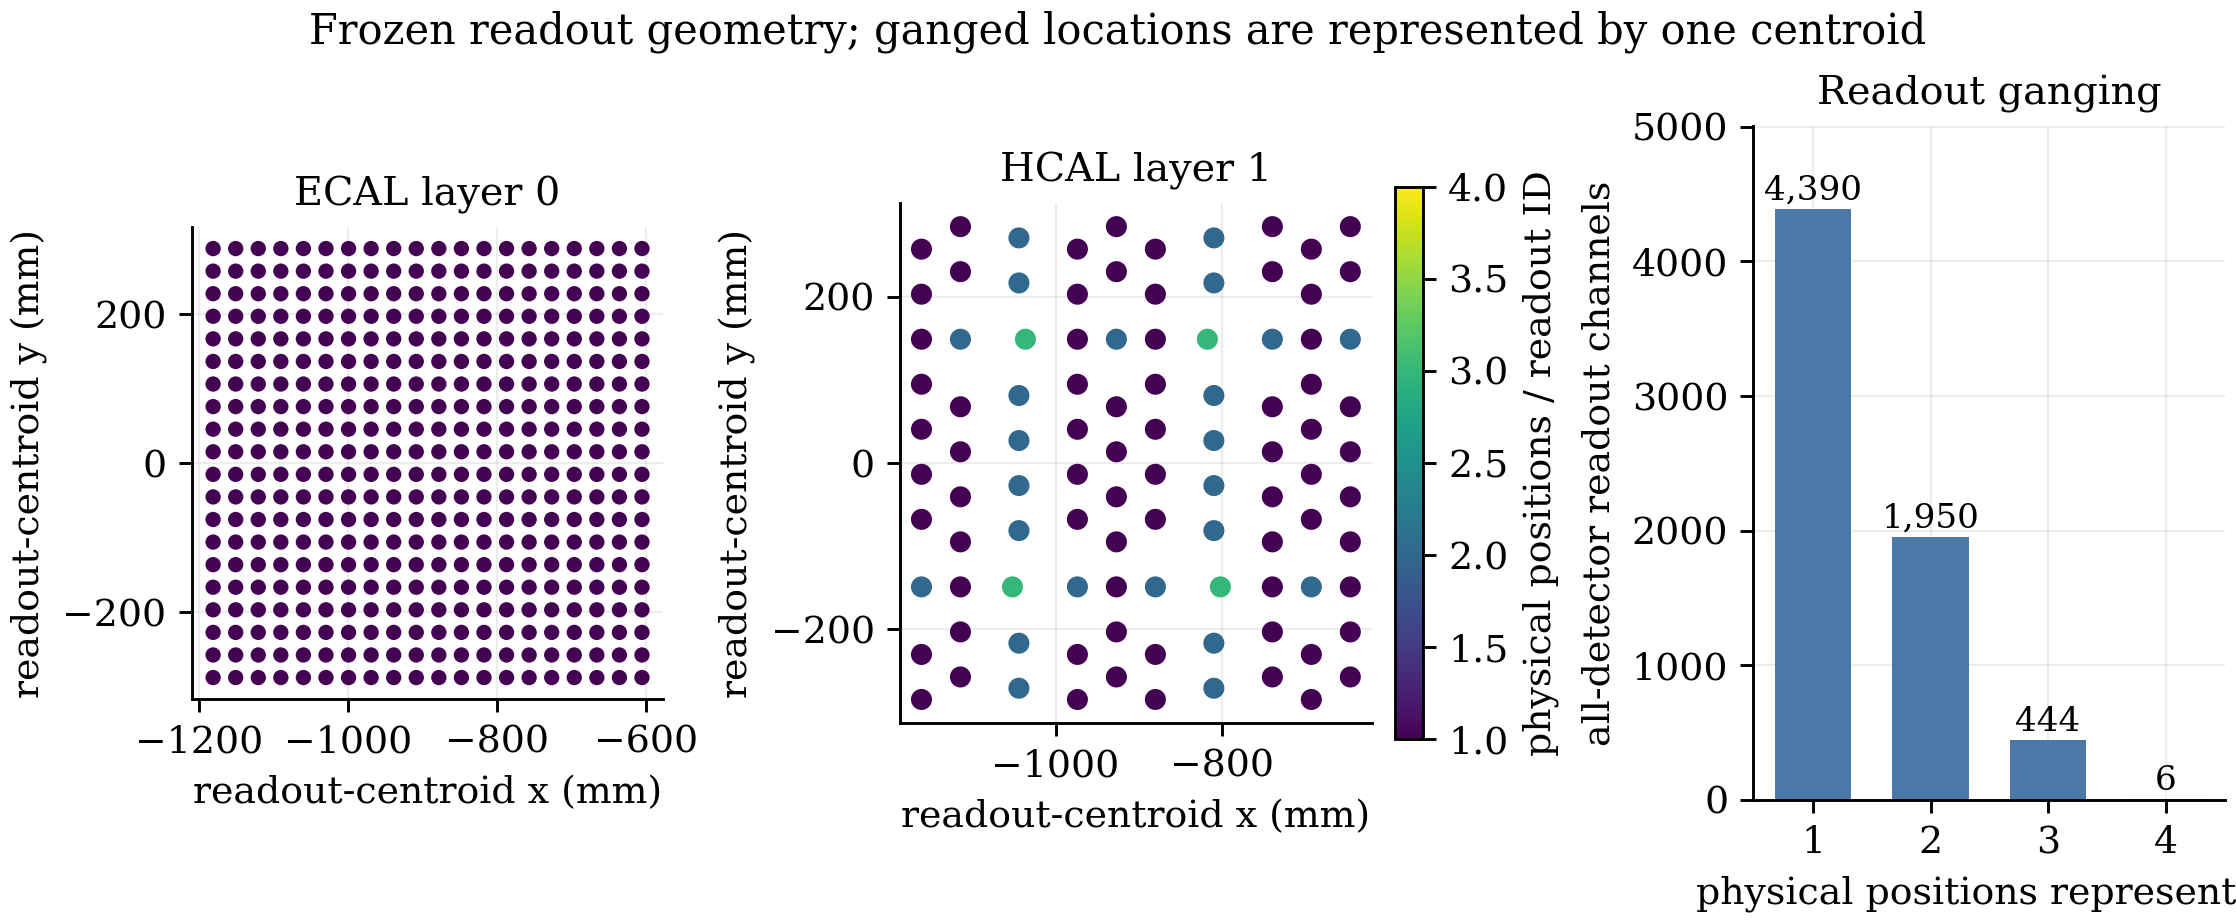
\includegraphics[width=\linewidth]{detector_geometry.png}
 \caption{Frozen readout geometry. The left panels show ECAL layer 0 and HCAL layer 1. The ganging histogram covers all 6,790 readout channels; its first bar contains 400 ECAL and 3,990 HCAL channels.}
 \label{fig:geometry}
\end{figure}

The graph connects every channel to its eight nearest same-layer centroids. For each node in layer $\ell=0,\ldots,63$, four nearest centroids are selected in layer $\ell+1$, and each selected longitudinal pair is stored in both directions. This gives $8\times6790=54{,}320$ lateral directed edges and $2\times4\times(400+63\times100)=53{,}600$ longitudinal directed edges, or 107,920 in total. The same graph is used by the generator and by the connectivity diagnostic. It is an implementation graph, not a uniquely established physical-neighbor graph, and centroiding removes separation within a ganged channel.

The preparation record contains 764,940 events over 0--300\,GeV, divided by deterministic event hash into 612,482 training, 76,158 validation, and 76,300 nominal test events. The checkpoint studied here used a smaller pilot of 26,624 training events and 6,656 validation events. Its training population is 4.35\% of the canonical training partition.

All shower comparisons use a 10,000-condition sample from the canonical validation partition with $50\leq\Kinc\leq250\GeV$. We call this sample $\Ddev$: it was inspected during model and manuscript development, and its overlap with the 6,656-event pilot-validation sample is not recoverable from the released aggregates. No nominal test event is used in this manuscript. The results are therefore descriptive measurements of the stored pairs, rather than an untouched assessment of expected model performance.

\section{Generator and training procedure}
\label{sec:model}

The generator has 2,082,507 trainable parameters. It receives only the five conditioning features in Eq.~\eqref{eq:condition}; no reference shower is supplied when an event is generated. A two-block residual multilayer perceptron maps the five inputs to a 128-component vector $h_c$. Every subsequent head is conditioned on $h_c$. The model is not an autoencoder: it has no learned shower encoder and no single latent vector shared by all stages. Randomness instead enters through the discrete draws and through separate Gaussian source states for the two conditional flows described below.

Figure~\ref{fig:architecture} follows the inference path. Each sampled quantity becomes an input to the next stage. This ordering defines the model's factorization: an error in an early draw can propagate downstream, whereas a later stage cannot alter an upstream budget or count.

\begin{center}
\begin{minipage}{\linewidth}
 \centering
 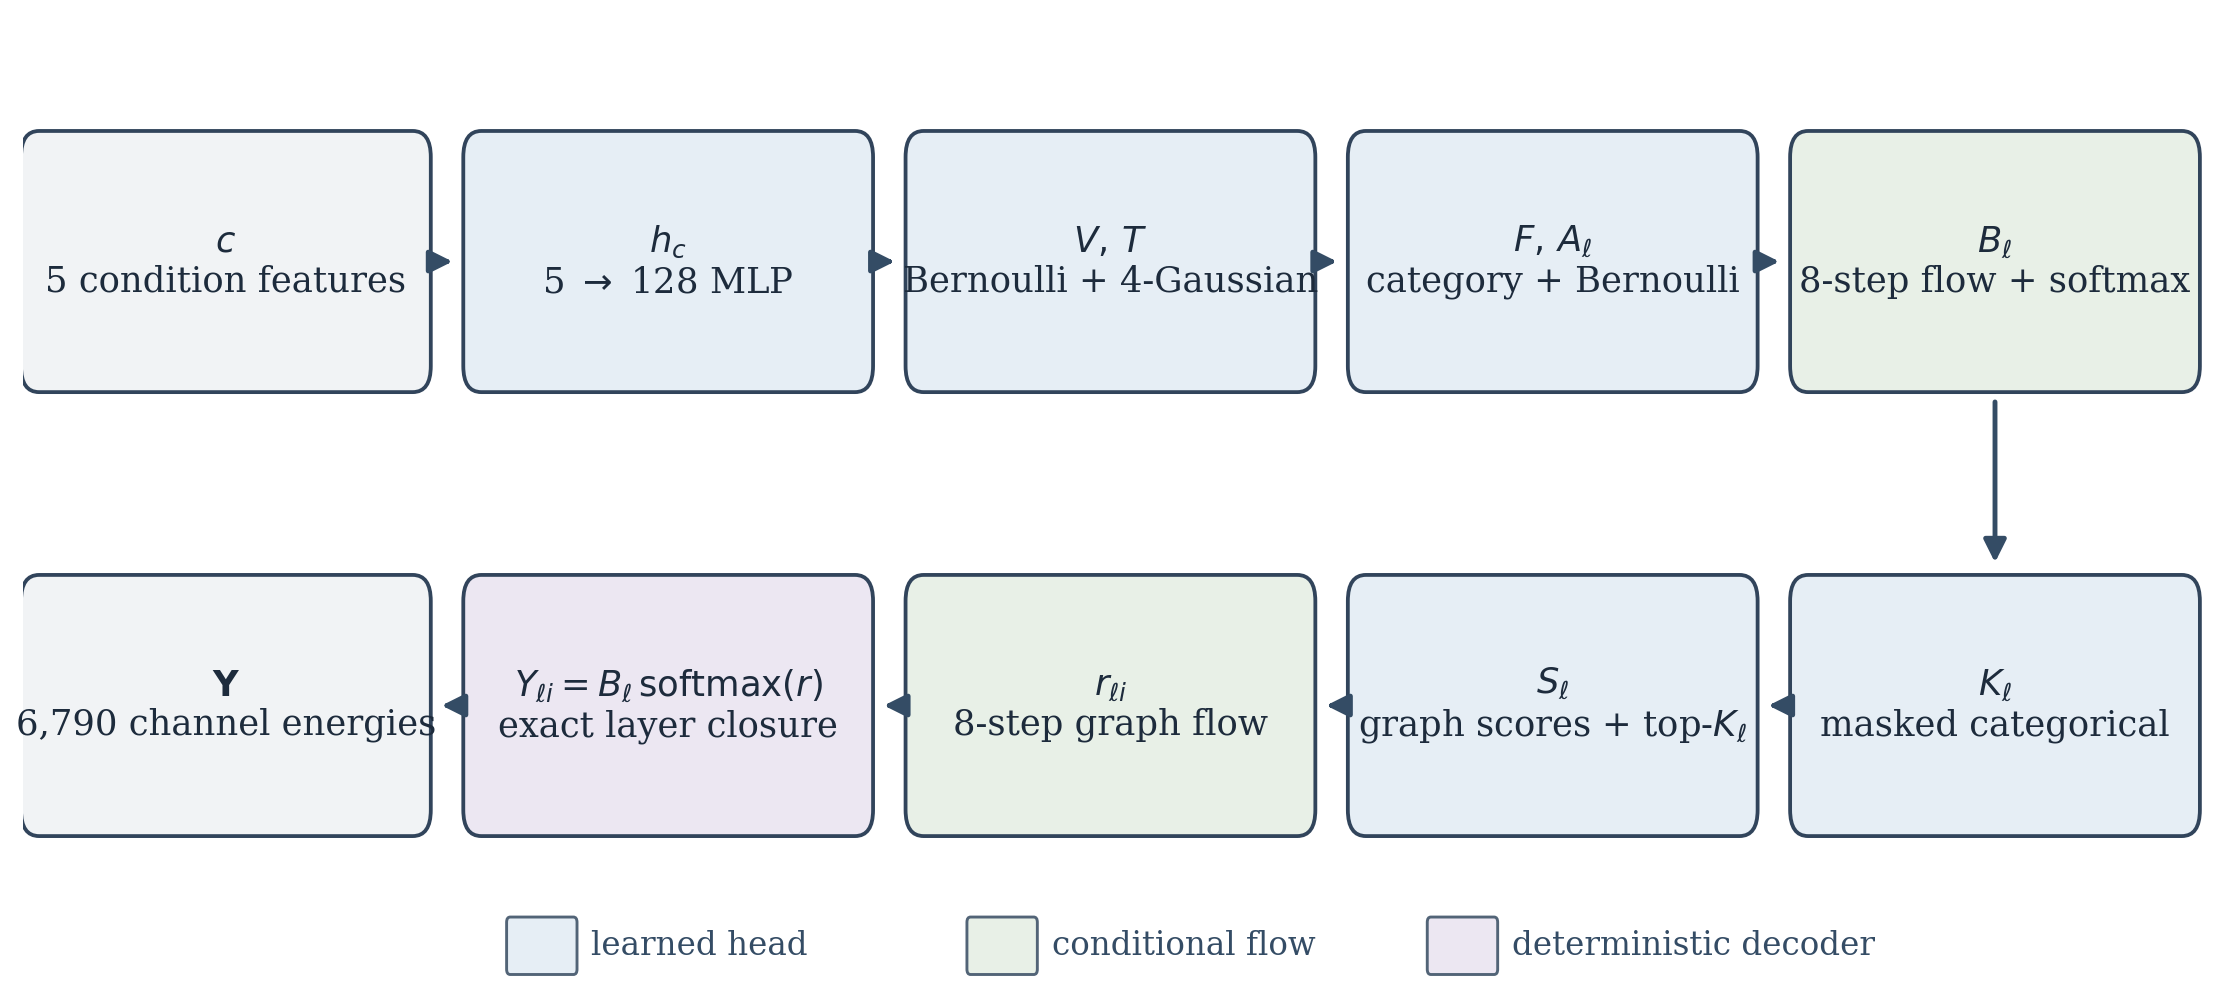
\includegraphics[width=\linewidth]{generator_schematic.png}
 \captionof{figure}{Event generation in sampling order. Blue boxes are learned probability heads, green boxes are conditional flow fields, and the purple box is a deterministic decoder. $V$ is the visible-event indicator, $T$ is total readout deposit, $F$ is the first active layer, $A_\ell$ is layer activity, $B_\ell$ is the layer budget, $K_\ell$ is the active-channel count, and $S_\ell$ is the selected support. During training, each head receives the corresponding quantities derived from the reference shower. During inference, it receives the sampled outputs of earlier stages.}
 \label{fig:architecture}
\end{minipage}
\end{center}

\subsection{Total deposit and longitudinal allocation}

A Bernoulli head samples the visible-event indicator $V$. A second head outputs the mixture weights, means, and positive scales of a four-component Gaussian mixture for
\begin{equation}
 q_T=\log(1+T/10\GeV).
 \label{eq:response_transform}
\end{equation}
When $V=1$, the implementation samples a mixture component and a normal variate, applies the inverse transform, and sets a negative result to zero. It then limits the result to
\begin{equation}
 0\leq T\leq C(\Kinc),\qquad
 C(\Kinc)=\min\{0.630110\max(\Kinc,1\GeV),61.2338\GeV\}.
 \label{eq:cap}
\end{equation}
The cap is a numerical bound derived from the training sample. If $V=0$, or if the transformed draw becomes zero after inversion and clipping, the implementation sets $T=0$ and generates no active layer. The aggregate evaluation did not retain cap-activation or reference-exceedance counts, so it cannot test the response tail near this boundary.

For $V=1$, a categorical head samples the first active layer $F$ from $(h_c,T)$. Layers before $F$ are set inactive, layer $F$ is forced active, and a Bernoulli head samples the later activity indicators. The later indicators are independent conditional on the variables supplied to that head,
\begin{equation}
 p(\mathbf A\mid h_c,T,F)=\prod_{\ell>F}^{64}p(A_\ell\mid h_c,T,F,\ell),
 \qquad A_F=1.
 \label{eq:activity}
\end{equation}
This head does not require the active layers to be contiguous.

The first conditional flow assigns the total deposit to the sampled active layers. Its training target is the centered log of the reference layer fractions after flooring each fraction at $10^{-8}$. For a transformed target $x_1$, flow training draws $x_0$ from a standard normal distribution and $t$ uniformly from $[0,1]$, constructs
\begin{equation}
 x_t=(1-t)x_0+t x_1,
 \qquad
 \mathcal L_{\mathrm{CFM}}=\lVert v_\theta(x_t,t;\text{context})-(x_1-x_0)\rVert_2^2,
 \label{eq:cfm}
\end{equation}
and fits the velocity field $v_\theta$ by mean-squared error~\cite{flowmatching}. At inference, the flow starts from a new Gaussian draw on the active layers and applies eight fixed first-order updates to the learned ordinary differential equation. A masked softmax then gives layer fractions $\pi_\ell$, and the layer budgets are
\begin{equation}
 B_\ell=T\pi_\ell,\qquad B_\ell=0\ \text{when}\ A_\ell=0,
 \qquad \sum_{\ell=0}^{64}B_\ell=T.
 \label{eq:layer_budget}
\end{equation}
The velocity field uses a 128-component layer representation and two bidirectional transformer layers with four attention heads. Its context comprises $h_c$, $T$, the sampled activity mask, layer identity, and a sinusoidal encoding of flow time.

\subsection{Channel count, support, and deposited energy}

For each layer, a categorical head receives $(h_c,B_\ell,A_\ell)$ and a learned layer embedding, then samples the number of active channels $K_\ell$. Its feasibility mask permits only $K_\ell=0$ in an inactive layer and $1\leq K_\ell\leq N_\ell$ in an active layer, where $N_\ell$ is the number of channels in that layer. Because this study uses a zero threshold, the count mask imposes no positive minimum energy per selected channel.

The support network assigns one score to every channel. Its static node inputs are standardized $(x,y,z)$ coordinates, normalized layer index, and ECAL/HCAL indicators. It appends $h_c$, the budget $B_\ell$, and the occupancy fraction $K_\ell/N_\ell$ for the channel's layer. Three 96-component message-passing blocks use the directed graph and five edge features: standardized coordinate differences, their Euclidean norm, and a code for lateral, forward-longitudinal, or backward-longitudinal edges. Node representations are then averaged within each layer; a two-layer, four-head bidirectional transformer exchanges information among the 65 layer summaries; and the resulting layer context is broadcast back to the nodes. Adding independent Gumbel noise to the scores and retaining the largest $K_\ell$ values selects exactly $K_\ell$ channels in layer $\ell$~\cite{gumbeltopk}. This operation fixes support cardinality, but it does not require the selected nodes to form a connected set.

The second conditional flow assigns relative energy within the selected support. Its target is the centered log of the reference channel fractions in each layer after the same $10^{-8}$ floor. It uses the construction in Eq.~\eqref{eq:cfm}. The velocity network has the same graph and layer-context structure as the support network, with the current flow state and a sinusoidal time encoding added to each node. Node states are masked by the selected support before and after every message-passing block. At inference, the selected nodes receive independent Gaussian source values, and eight fixed first-order updates produce final logits $r_{\ell i}$. The deterministic decoder computes
\begin{equation}
 Y_{\ell i}=
 \begin{cases}
 B_\ell\,\dfrac{\exp r_{\ell i}}{\sum_{j\in S_\ell}\exp r_{\ell j}}, & i\in S_\ell,\\[6pt]
 0, & i\notin S_\ell,
 \end{cases}
 \label{eq:decoder}
\end{equation}
where $S_\ell$ is the selected set. Thus, in exact arithmetic, $|S_\ell|=K_\ell$, $Y_{\ell i}\geq0$, $\sum_iY_{\ell i}=B_\ell$, and $\sum_{\ell i}Y_{\ell i}=T$. These identities conserve the model's sampled readout budget. They do not enforce conservation of incident-neutron energy, agreement with Geant4, or connectivity of the selected support.

\subsection{Training and checkpoint selection}

Training uses the reference shower to derive $V$, $T$, $F$, $A_\ell$, $B_\ell$, $K_\ell$, $S_\ell$, and the two flow targets. Each component is trained with those reference upstream quantities rather than with samples from preceding heads; this is the teacher forcing shown in Fig.~\ref{fig:architecture}. The nine losses are binary cross entropy for visibility and activity, mixture negative log likelihood for $T$, categorical cross entropy for $F$ and $K_\ell$, binary cross entropy plus pairwise ranking for support, and mean-squared velocity error for each flow. Their weights were obtained from gradient norms measured on training data. Response, layer-profile, and count weights reached the lower clipping bound, while the visibility weight reached the upper bound; this records the optimizer setup and does not identify the source of the connectivity discrepancy.

The selected joint-training run used AdamW with a peak learning rate of $3\times10^{-4}$, batch size six, accumulation over four batches, gradient clipping at one, and seed 20260723. Epoch 90 has the lowest recorded validation objective among the 104 retained rows spanning epochs 11--114 and defines the checkpoint studied here. Validation objectives are lower than training objectives over much of this record. The retained aggregates do not identify why, so the ordering is not given a physical interpretation. Both flows use eight integration updates at evaluation; no solver-step comparison was retained.

\section{Diagnostics}
\label{sec:diagnostics}

We first compare all-event mean total, ECAL, and HCAL deposits. Eight 25\,GeV incident-energy bins are also available as aggregate means and standard deviations. They are used only to identify the range of descriptive deviations because the retained report contains no binwise uncertainty estimates. We omit the pooled Wasserstein distance and the historical reference-half comparison: the sample sizes and condition distributions differ, and the stored bootstrap does not provide a calibrated uncertainty statement for that comparison.

A layer or channel is active when its stored energy is strictly positive; no detector or analysis threshold is applied. For a nonempty event with first and last active layers $F$ and $L$, the occupied span is $L-F+1$, and the number of inactive layers inside it is
\begin{equation}
 G=L-F+1-\sum_{\ell=0}^{64}A_\ell.
 \label{eq:gaps}
\end{equation}
This counts inactive layers, not contiguous runs. A shower has an interior gap when $G>0$. On the undirected form of the model graph, the active support $S$ separates into weak components $C_1,\ldots,C_m$; we report $m$ and $\max_j|C_j|/|S|$. All support summaries are conditioned on nonempty events. The reference and generated nonempty sample sizes are 9,907 and 9,858, respectively.

The retained condition-only pipeline control has AUROC 0.500. Because it contains no shower variables, it checks only that identical condition distributions are presented to the two labels; it is not a two-sample test of the generated showers. A valid classifier test would require held-out discrimination~\cite{kansalmetrics} and, for this paired design, a split that keeps each matched reference--generated pair together.

\section{Results}
\label{sec:results}

Table~\ref{tab:results} reports absolute differences so that ratios on small denominators do not exaggerate the comparison. The all-event mean total deposit differs by 0.045\,GeV, but this sum combines an ECAL excess of 0.175\,GeV with an HCAL deficit of 0.129\,GeV. Across the eight incident-energy bins, the generated-minus-reference mean difference ranges from $-7.7\%$ to $+7.7\%$, while the standard-deviation difference ranges from $-10.9\%$ to $+9.6\%$. Without binwise uncertainties these ranges diagnose possible cancellation but do not establish a statistically resolved energy dependence.

\begin{table}[t]
\centering
\caption{Aggregate development-bank results. Deposit rows and zero-deposit counts use all 10,000 pairs. Support rows are conditional on nonempty events (9,907 reference and 9,858 generated). Percentage-point differences are denoted pp. No uncertainty intervals can be reconstructed from the retained aggregates.}
\label{tab:results}
\small
\begin{tabular}{@{}lrrr@{}}
\toprule
Quantity & Geant4 reference & Generator & Gen. $-$ ref. \\
\midrule
Zero-deposit events & 93 (0.93\%) & 142 (1.42\%) & $+49$ ($+0.49$ pp) \\
Mean total deposit (GeV) & 4.324 & 4.369 & $+0.045$ \\
Mean ECAL deposit (GeV) & 2.100 & 2.275 & $+0.175$ \\
Mean HCAL deposit (GeV) & 2.224 & 2.094 & $-0.129$ \\
\midrule
Mean first active layer & 0.510 & 0.735 & $+0.225$ \\
Mean last active layer & 56.20 & 60.62 & $+4.42$ \\
Mean active layers & 54.58 & 54.83 & $+0.25$ \\
Mean occupied span & 56.69 & 60.88 & $+4.20$ \\
Mean inactive layers in span & 2.10 & 6.05 & $+3.95$ \\
Events with an interior gap & 52.43\% & 93.53\% & $+41.10$ pp \\
Mean active channels & 1617.6 & 1588.8 & $-28.7$ \\
Mean weak graph components & 23.42 & 59.39 & $+35.97$ \\
Mean largest-component fraction & 94.90\% & 88.87\% & $-6.03$ pp \\
\bottomrule
\end{tabular}
\end{table}

The longitudinal discrepancy is more directly described as a shift in reach than as a ratio of gap counts. The generated shower has nearly the same mean number of active layers, but its first active layer is 0.225 layer later and its last active layer is 4.42 layers later. The occupied span consequently grows by 4.20 layers while the active-layer count grows by only 0.25, leaving 3.95 additional inactive layers inside the span. Figure~\ref{fig:longitudinal} shows the corresponding mean energy allocation.

\begin{figure}[t]
 \centering
 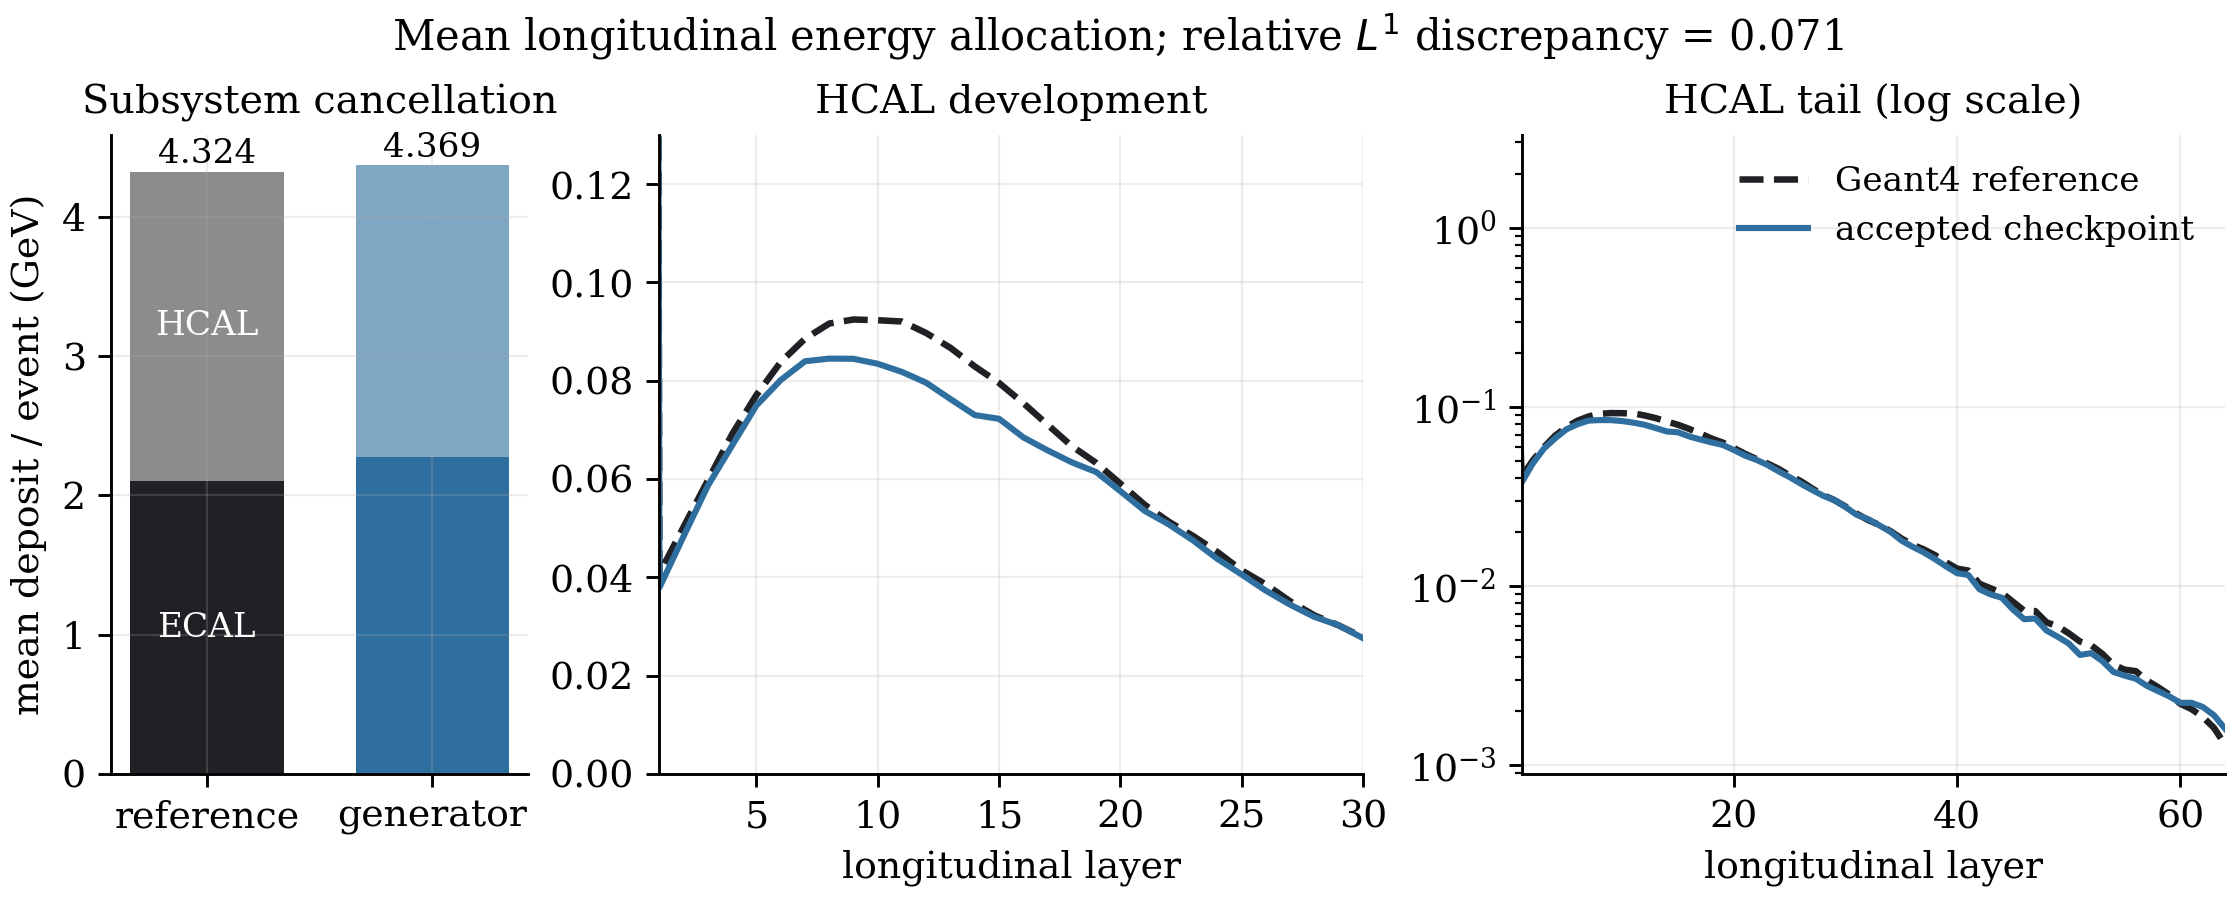
\includegraphics[width=\linewidth]{longitudinal_profile.png}
 \caption{Mean longitudinal allocation on $\Ddev$. The stacked bars expose the opposing ECAL and HCAL shifts. The layer panels show HCAL layers only; ECAL layer 0 is isolated in the bars. The curves are descriptive means without event-level uncertainty bands.}
 \label{fig:longitudinal}
\end{figure}

At channel level, the generated events contain 28.7 fewer active channels on average but 35.97 more weak components. Their largest component contains 6.03 percentage points less of the active support. Under the declared graph and strict-positive definition, the support is therefore more disconnected even though its mean cardinality is similar. The available aggregates do not record component energies. They cannot determine whether the additional components carry substantial energy or arise from small positive deposits produced by the selected-channel softmax.

There are 49 more zero-deposit generated events than reference events. A significance calculation would require the joint paired zero/nonzero counts, which were not retained; the marginal counts alone do not support one. The result is reported because the visibility hurdle is part of the sampled model and because excluding empty events changes the denominators of every support statistic.

The decoder-level checks passed for all 1,250 batches of eight generated events. No nonfinite value, negative value, invalid support, requested-versus-realized count mismatch, or positive-support mismatch was recorded. Maximum event and layer budget residuals were $1.14\times10^{-5}$ and $3.05\times10^{-5}$\,GeV under the evaluator's batch-wide absolute-plus-relative tolerance. These checks establish consistency with sampled budgets and counts for this generated bank; they do not test agreement with Geant4.

\section{Discussion}
\label{sec:discussion}

The empirical statement supported by these aggregates is specific: one pilot checkpoint produces a later and more disconnected strict-positive readout support than its paired Geant4 sample while retaining similar mean layer and channel multiplicities. Exact cardinality and budget allocation leave the spatial arrangement underdetermined, so this coexistence is compatible with the decoder construction. The comparison does not show that the factorization caused the discrepancy. Limited training data, checkpoint selection, numerical integration, the shared graph, and the zero threshold remain alternative explanations.

Connectivity is one useful projection of shower structure, but it is not a complete or representation-independent fidelity metric. CaloChallenge and CaloDREAM illustrate the broader practice of combining one-dimensional shower observables with multivariate diagnostics~\cite{calochallenge,calodream}. The HEP metric literature similarly recommends complementary tests rather than a single scalar ranking~\cite{kansalmetrics}. For this readout, a defensible connectivity result would additionally require thresholds tied to detector noise or digitization, energy-weighted component summaries, alternative adjacency graphs, and distributions resolved in incident energy and direction.

Several additional tests are needed because they answer different questions. Repeating generation with several sampling seeds would measure Monte Carlo variability for the fixed checkpoint. Neighboring checkpoints and independent training seeds would test selection and training variability. A 26k--100k--full-data scaling study would test whether the result changes with training-set size. Replacing generated upstream variables with their reference counterparts in an oracle cascade would show where the discrepancy first appears in the hierarchy. Solver-step scans would test numerical integration. Matched alternatives for layer activity and support selection would test whether those design choices alter connectivity. The present aggregate file cannot supply any of these comparisons.

$\Ddev$ was repeatedly inspected, its overlap with pilot validation is unresolved, and event-level arrays were not retained. A physics-performance paper would require a locked evaluation bank with documented identities, paired uncertainty estimates, full structural distributions, a valid shower-aware classifier test, reconstructed-observable comparisons, and end-to-end timing. A complete reference-simulation specification and the applicable collaboration approval would also be required. The present evidence therefore supports an exploratory computational-physics case study, but not a validated fast-simulation result.

\section{Conclusion}

For the single pilot checkpoint studied here, close mean occupancies do not coincide with close readout-support organization. Relative to the paired Geant4 sample, the generated events contain 0.25 more active layers but reach 4.42 layers farther downstream, leaving 3.95 more inactive layers within the occupied span. They contain 28.7 fewer active channels but 35.97 more weak components on the model graph, with a 6.03-percentage-point reduction in the largest-component fraction. Opposing ECAL and HCAL shifts also partially cancel in the mean total deposit.

These values describe one repeatedly inspected development bank under a strict-positive threshold and one shared graph. They establish a reproducible discrepancy in this artifact. They do not establish its statistical significance, physical relevance after digitization, persistence across model fits, or causal origin. Those questions require the event-level, threshold, graph, seed, and locked-evaluation studies specified above.

\section*{Code and data availability}

The manuscript source, aggregate validation report, event-independent geometry summary, training-history extract, figure builder, and QA records are available at \url{https://github.com/JulianAttemptsCoding/fast-mc-paper}. The collaboration-owned event file and checkpoint are not redistributed. The public package reproduces the manuscript and aggregate arithmetic; it cannot retrain the model, regenerate showers, or reconstruct event-level tests.

\section*{Acknowledgments}

The author thanks Dr. Wen-Chen Chang (Institute of Physics, Academia Sinica) for mentorship and guidance on the experimental high-energy-physics context of this project.

\section*{Author contributions}

Julian Juan: conceptualization, methodology, software, investigation, visualization, and writing.

\section*{Use of generative AI}

Generative-AI tools were used for editorial assistance, code generation, literature discovery, and adversarial manuscript auditing. Numerical statements were checked against versioned project artifacts during this revision; the author retains responsibility for verifying and approving the final manuscript.

\printbibliography

\end{document}
